\chapter{El simulador}
\label{ch:simulador}

El simulador se construyó utilizando la librería Qutip 4.2 de Python 3.6. Esta es una librería que incluye varias herramientas para realizar simulaciones de sistemas mecánico cuánticos, entre ellas, un solucionador de ecuaciones maestras. El funcionamiento básico del simulador desarrollado es el siguiente:

\begin{enumerate}
    \item Leer estado inicial
    \item Construir Hamiltoniano del sistema
    \item Introducir Hamiltoniano y estado inicial en el solucionador de ecuaciones maestras.
    \item Retornar solución
\end{enumerate}

De esta manera se simulan las compuertas naturales de los transmones. Luego, a partir de estas se construyen todas las demás compuertas que se necesitaran para construir un conjunto de compuertas cuánticas con el cual poder ejecutar los algoritmos de Grover, Shor y PageRank.

Se simularon dos sistemas distintos, uno de cuatro qubits y otro de ocho qubits. El diseño original era el de cuatro qubits, con él se realizaron las simulaciones del algoritmo de Grover y del PageRank. Sin embargo, el algoritmo de Shor requiere de al menos ocho qubits para factorizar el número compuesto impar más pequeño: el número 15. Posteriormente también se realizo una generalización del simulador para poder trabajar con sistemas de n qubits.

El tipo de acoplamiento entre los qubits elegido es el acoplamiento de tipo bus. De esta manera trabajamos con un único resonador, el cual se puede tracear. Esto reduce significativamente la dimensión del sistema a simular y nos permite tener más qubits. Además, de esta forma, la interación es más directa y basta con la compuerta iSWAP para construir cualquier otra compuerta multiqubits, el cual no sería el caso con qubits acoplados a distintos resonadores, pues se necesitarían compuertas de interacción entre resonadores.

\section{Parámetros de los sistemas simulados}

Se han elegido parámetros típicos de los sistemas de qubits\cite{blais}.

\begin{enumerate}
    \item Frecuencias de resonancia:
        \begin{enumerate}
            \item Resonador: 10GHz
            \item Qubit 0: 5GHz
            \item Qubit 1: 6GHz
            \item Qubit 2: 7GHz
            \item Qubit 3: 8GHz
            \item *Qubit 4: 11GHz
            \item *Qubit 5: 12GHz
            \item *Qubit 6: 13GHz
            \item *Qubit 7: 14GHz
        \end{enumerate}
    \item Constante de acoplamiento: Todas iguales a 0.1GHz
    \item Tasas de relajación: Todas iguales a 25KHz
    \item Tiempo de relajación: Todos iguales a $40 \mu s$
    \item Frecuencia de resonancia para iSWAP: 9GHz
\end{enumerate}

*Sólo aplica para el caso del sistema de 8 qubits

\section{Compuertas nativas}

Como se vio en el capítulo anterior, en los transmones se puede ejecutar de manera natural las compuertas Rx, Ry e iSWAP. Estas compuertas se implementan en el simulador y es a partir de ellas que se contruyen todas las demás.

\begin{equation}
    H_{R_x} = -\frac{1}{2} \sum\limits_i \Delta_{q_i} \sigma_{z_i} + \xi(t) \sigma_{x_{target}}
\end{equation}

\begin{equation}
    H_{R_y} = -\frac{1}{2} \sum\limits_i \Delta_{q_i} \sigma_{z_i} + \xi(t) \sigma_{y_{target}}
\end{equation}

\begin{equation}
    H_{iSWAP} = \frac{g_1 g_2}{\Delta_{swap}} (\sigma_{+_1} \sigma_{-_2} + \sigma_{-_1} \sigma_{+_2})
\end{equation}

\subsection{Rx y Ry}

Estas compuertas se logran realizan un pulso gaussiano de microondas en fase (Rx) o en cuadratura (Ry). Se han elegido pulsos de 10ns de duración, truncados en $\pm 3 \sigma$.

\begin{equation}
    \xi(t) = A \Pi\left(\frac{t-\mu}{6\sigma}\right) \frac{1}{\sqrt{2 \pi \sigma^2}} e^{-\frac{(x-\mu)^2}{2 \sigma^2}}
\end{equation}

Donde $\mu = 5ns$, $\sigma = \frac{5}{3} ns$, $\Pi(t)$ es la función rectangular, $A = \frac{\theta}{N}$ y $N = 0.9973$ es una constante de normalización. De esta manera se tiene el pulso gaussiano truncado deseado de 0ns a 10ns, cuya área bajo la curva sea igual al ángulo $\theta$ de la rotación.

\begin{figure}[H]
    \centering
    \begin{subfigure}[m]{0.49\textwidth}
        \centering 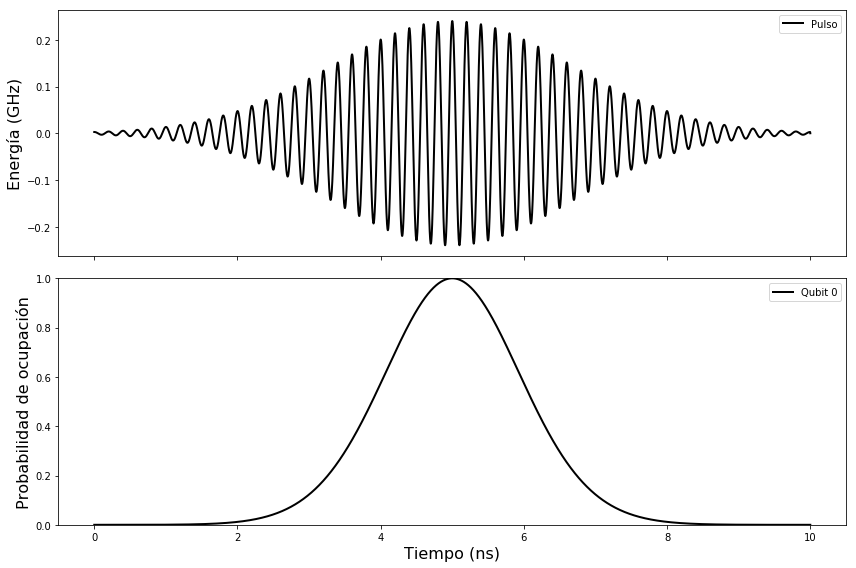
\includegraphics[width=1\linewidth]{img/rx02pi.png}
        \caption{Rx}
    \end{subfigure}
    \begin{subfigure}[m]{0.49\textwidth}
        \centering 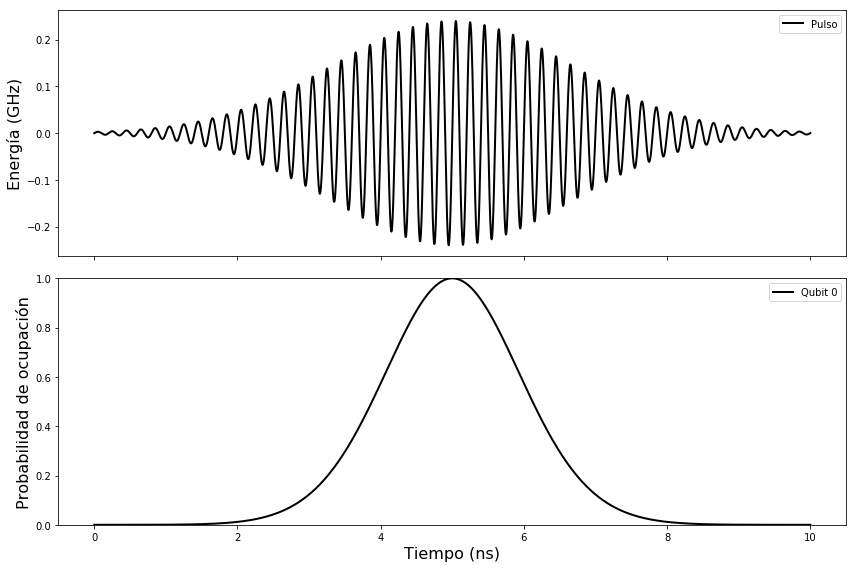
\includegraphics[width=1\linewidth]{img/ry02pi.png}
        \caption{Ry}
    \end{subfigure}
    \caption[Rotaciones en X e Y de $2\pi$]{Rotaciones en X e Y de $2\pi$}
\label{fig:rxry02pi}
\end{figure}

\begin{figure}[H]
    \centering
    \begin{subfigure}[m]{0.49\textwidth}
        \centering 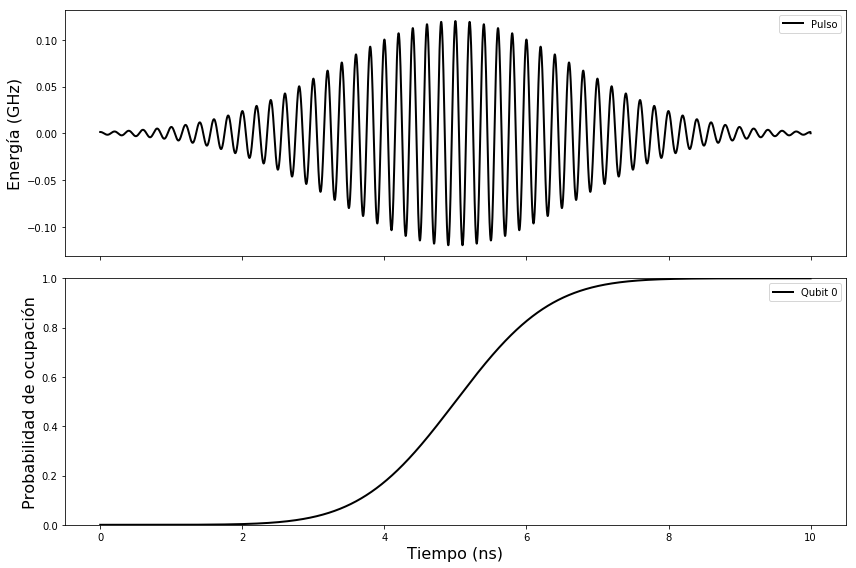
\includegraphics[width=1\linewidth]{img/rx0pi.png}
        \caption{Rx}
    \end{subfigure}
    \begin{subfigure}[m]{0.49\textwidth}
        \centering 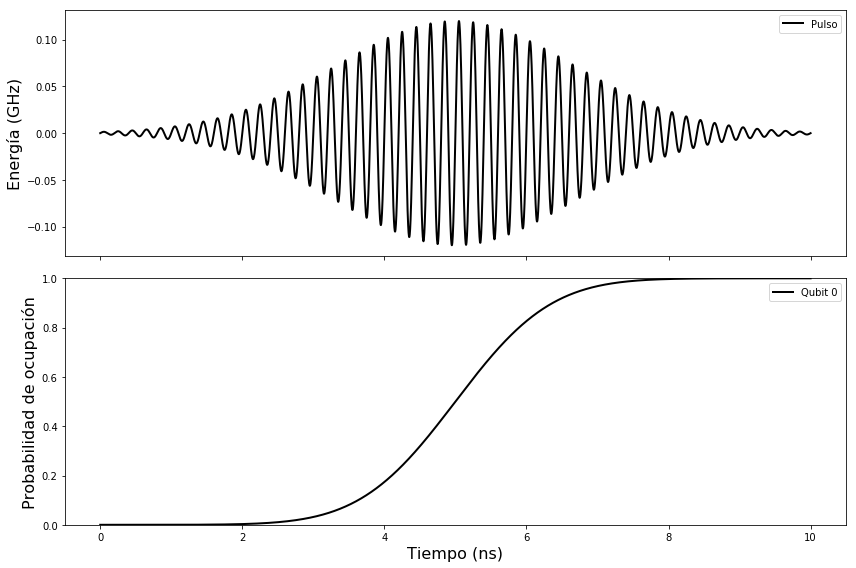
\includegraphics[width=1\linewidth]{img/ry0pi.png}
        \caption{Ry}
    \end{subfigure}
    \caption[Rotaciones en X e Y de $\pi$]{Rotaciones en X e Y de $\pi$}
\label{fig:rxry0pi}
\end{figure}

\begin{figure}[H]
    \centering
    \begin{subfigure}[m]{0.49\textwidth}
        \centering 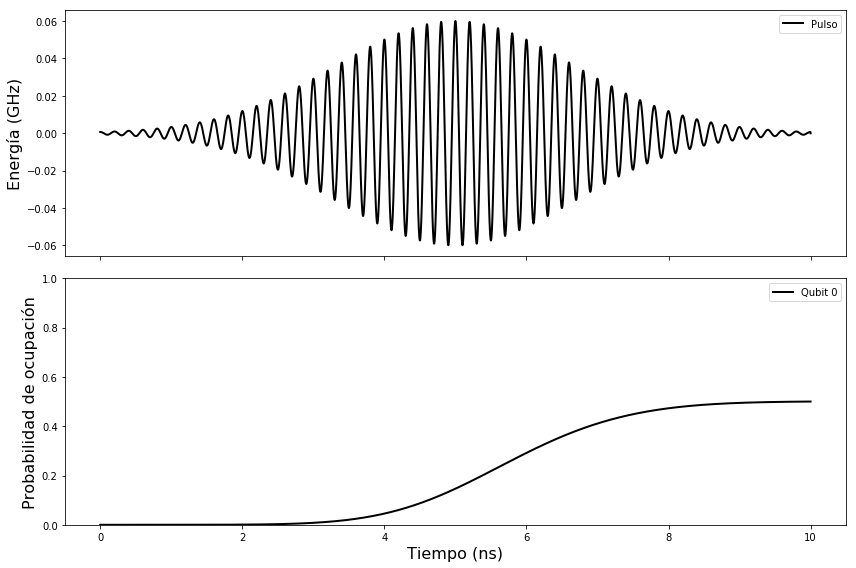
\includegraphics[width=1\linewidth]{img/rx0pi2.png}
        \caption{Rx}
    \end{subfigure}
    \begin{subfigure}[m]{0.49\textwidth}
        \centering 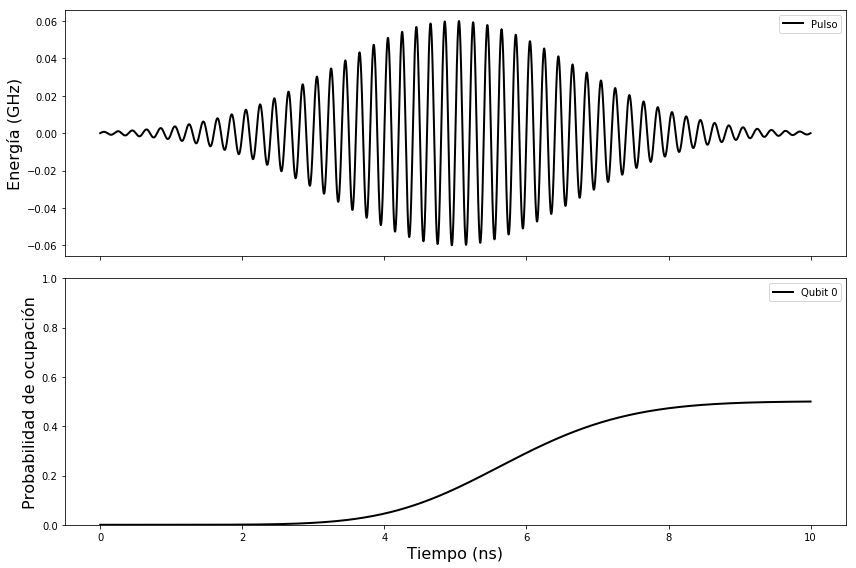
\includegraphics[width=1\linewidth]{img/ry0pi2.png}
        \caption{Ry}
    \end{subfigure}
    \caption[Rotaciones en X e Y de $\frac{\pi}{2}$]{Rotaciones en X e Y de $\frac{\pi}{2}$}
\label{fig:rxry0pi2}
\end{figure}

\subsection{iSWAP}

Esta compuerta se logra aplicando un campo magnético tal que la frecuencia de resonancia de los dos qubits deseados se mueva a $\omega_{swap} = 9GHz$. Esta interacción se deja durante $\frac{\pi}{2 J}$, donde $J = \abs{\frac{g_1 g_2}{\Delta_{swap}}}$ y $\Delta_{swap} = \omega_{swap} - \omega_r$. Esto es, esta interacción se deja por 25ns.

Si se desea realizar la compuerta $\sqrt{iSWAP}$, se debe dejar la misma interacción por sólo 12.5ns, que es la mitad del tiempo.

\begin{figure}[H]
    \centering
    \begin{subfigure}[m]{0.49\textwidth}
        \centering 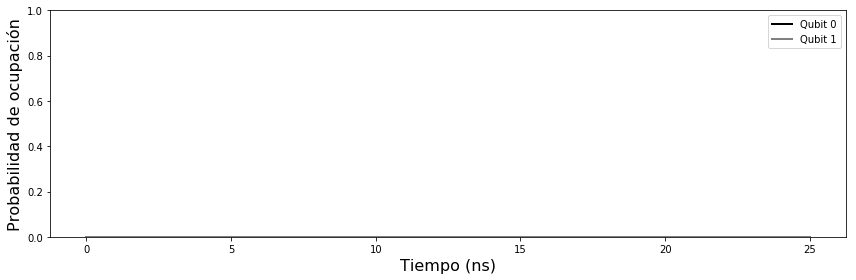
\includegraphics[width=1\linewidth]{img/iswap00.png}
        \caption{iSWAP}
    \end{subfigure}
    \begin{subfigure}[m]{0.49\textwidth}
        \centering 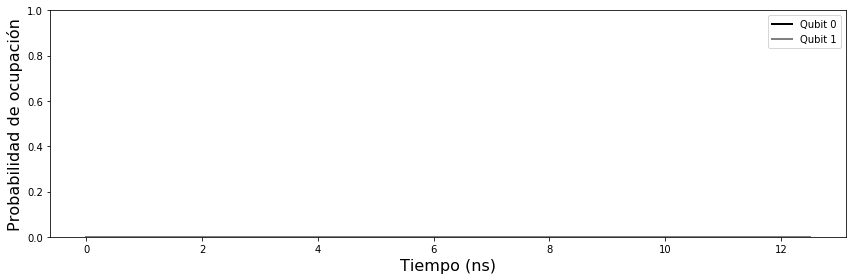
\includegraphics[width=1\linewidth]{img/sqrtiswap00.png}
        \caption{$\sqrt{iSWAP}$}
    \end{subfigure}
    \caption[Compuertas iSWAP y $\sqrt{iSWAP}$ aplicadas a $\ket{00}$]{Compuertas iSWAP y $\sqrt{iSWAP}$ aplicadas a $\ket{00}$}
\label{fig:iswapsqrtiswap00}
\end{figure}

\begin{figure}[H]
    \centering
    \begin{subfigure}[m]{0.49\textwidth}
        \centering 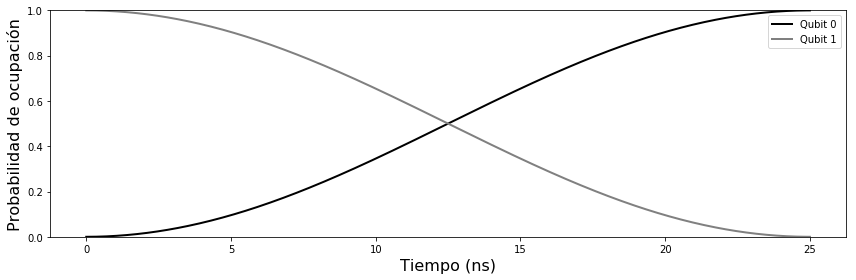
\includegraphics[width=1\linewidth]{img/iswap01.png}
        \caption{iSWAP}
    \end{subfigure}
    \begin{subfigure}[m]{0.49\textwidth}
        \centering 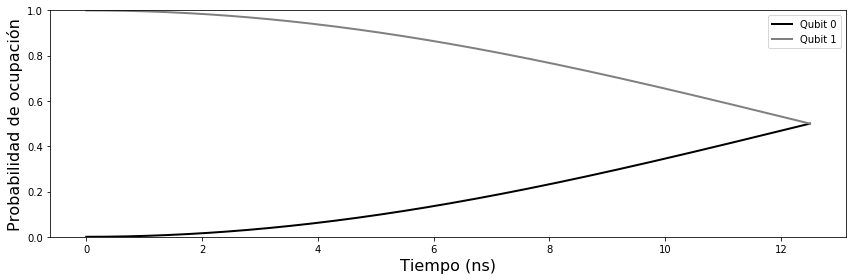
\includegraphics[width=1\linewidth]{img/sqrtiswap01.png}
        \caption{$\sqrt{iSWAP}$}
    \end{subfigure}
    \caption[Compuertas iSWAP y $\sqrt{iSWAP}$ aplicadas a $\ket{01}$]{Compuertas iSWAP y $\sqrt{iSWAP}$ aplicadas a $\ket{01}$}
\label{fig:iswapsqrtiswap01}
\end{figure}

\begin{figure}[H]
    \centering
    \begin{subfigure}[m]{0.49\textwidth}
        \centering 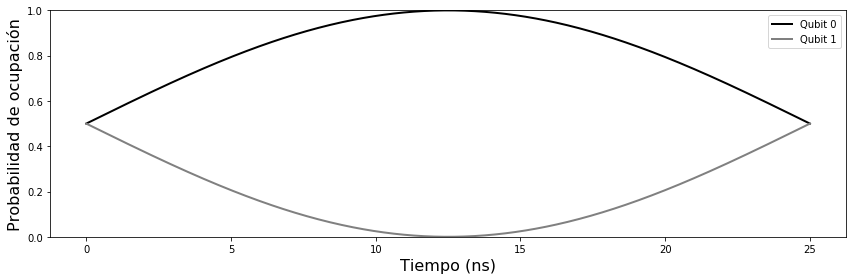
\includegraphics[width=1\linewidth]{img/iswap0011.png}
        \caption{iSWAP}
    \end{subfigure}
    \begin{subfigure}[m]{0.49\textwidth}
        \centering 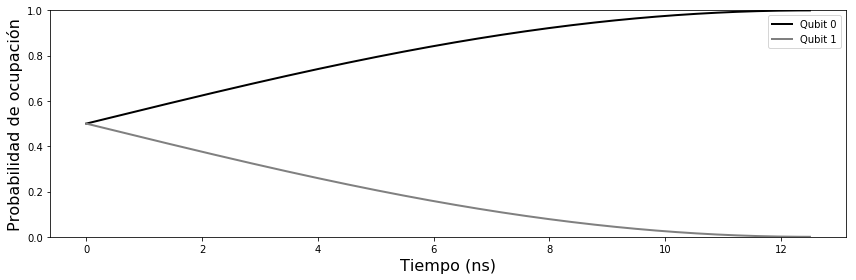
\includegraphics[width=1\linewidth]{img/sqrtiswap0011.png}
        \caption{$\sqrt{iSWAP}$}
    \end{subfigure}
    \caption[Compuertas iSWAP y $\sqrt{iSWAP}$ aplicadas a $\frac{\ket{00} + \ket{11}}{\sqrt{2}}$]{Compuertas iSWAP y $\sqrt{iSWAP}$ aplicadas a $\frac{\ket{00} + \ket{11}}{\sqrt{2}}$}
\label{fig:iswapsqrtiswap0011}
\end{figure}

\begin{figure}[H]
    \centering
    \begin{subfigure}[m]{0.49\textwidth}
        \centering 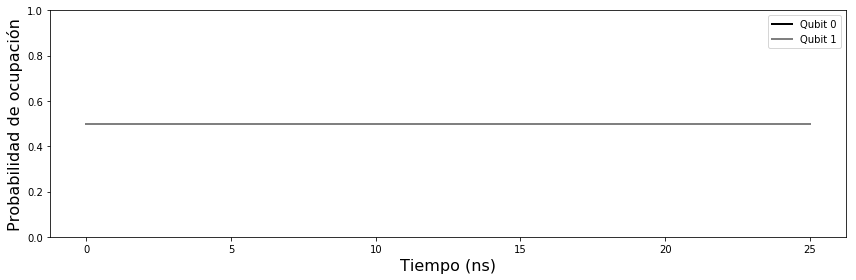
\includegraphics[width=1\linewidth]{img/iswap0101.png}
        \caption{iSWAP}
    \end{subfigure}
    \begin{subfigure}[m]{0.49\textwidth}
        \centering 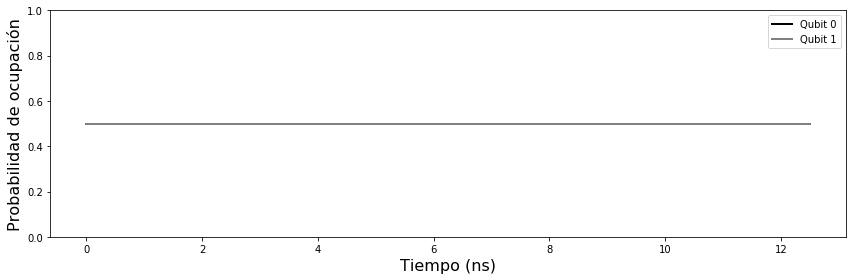
\includegraphics[width=1\linewidth]{img/sqrtiswap0101.png}
        \caption{$\sqrt{iSWAP}$}
    \end{subfigure}
    \caption[Compuertas iSWAP y $\sqrt{iSWAP}$ aplicadas a $\frac{\ket{0} + \ket{1}}{\sqrt{2}} \otimes \frac{\ket{0} + \ket{1}}{\sqrt{2}}$]{Compuertas iSWAP y $\sqrt{iSWAP}$ aplicadas a $\frac{\ket{0} + \ket{1}}{\sqrt{2}} \otimes \frac{\ket{0} + \ket{1}}{\sqrt{2}}$}
\label{fig:iswapsqrtiswap0101}
\end{figure}

\section{Compuertas compuestas}

Las compuertas anteriores forman un conjunto universal de compuertas cuánticas. A partir de secuencias de rotaciones en X e Y se puede formar cualquier rotación sobre cualquier eje de la esfera de Bloch, es decir, se puede realizar cualquier compuerta de un qubit. Con esto y cualquier compuerta de entrelazamiento, en nuestro caso $\sqrt{iSWAP}$, se tiene un conjunto universal de compuertas cuánticas y se puede realizar cualquier otra compuerta a partir de ellas.

\subsection{X}

Como tenemos $Rx(\theta)$, basta con hacer $\theta = \pi$ para realizar X, módulo una fase global de $-i$.

\begin{equation}
    X = 
    \begin{pmatrix}
        \cos(\frac{\pi}{2}) & -i \sin(\frac{\pi}{2}) \\
        -i \sin(\frac{\pi}{2}) & \cos(\frac{\pi}{2})
    \end{pmatrix} =
    \begin{pmatrix}
        0 & -i \\
        -i & 0
    \end{pmatrix} = 
    -i \begin{pmatrix}
        0 & 1 \\
        1 & 0
    \end{pmatrix}
\end{equation}

\subsection{Y}

Como tenemos $Ry(\theta)$, basta con hacer $\theta = \pi$ para realizar Y, módulo una fase global de $-i$.

\begin{equation}
    Y = 
    \begin{pmatrix}
        \cos(\frac{\pi}{2}) & -\sin(\frac{\pi}{2}) \\
        \sin(\frac{\pi}{2}) & \cos(\frac{\pi}{2})
    \end{pmatrix} =
    \begin{pmatrix}
        0 & -1 \\
        1 & 0
    \end{pmatrix} = 
    -i \begin{pmatrix}
        0 & -i \\
        i & 0
    \end{pmatrix}
\end{equation}

\[
\Qcircuit @C=1.4em @R=1.8em {
& \qw & \gate{X} & \qw 
}\]
\[\Qcircuit @C=1.4em @R=1.8em {
& \qw & \gate{Rx({\pi})} & \qw 
}
\]

\subsection{Rz}

Esta compuerta se realiza aplicando una transformación a Rx tal que el eje de rotación se rote y coincida con el eje Z. Es decir, el eje X se rota $\pi/2$ alrededor de Y:

\begin{multline}
    Rz(\theta) = Ry(\frac{-\pi}{2}) Rx(\theta) Ry(\frac{\pi}{2}) \\ =
    \begin{pmatrix}
        \frac{1}{\sqrt{2}} & \frac{1}{\sqrt{2}} \\
        -\frac{1}{\sqrt{2}} & \frac{1}{\sqrt{2}}
    \end{pmatrix}
    \begin{pmatrix}
        \cos(\frac{\theta}{2}) & -i \sin(\frac{\theta}{2}) \\
        -i \sin(\frac{\theta}{2}) & \cos(\frac{\theta}{2})
    \end{pmatrix}
    \begin{pmatrix}
        \frac{1}{\sqrt{2}} & -\frac{1}{\sqrt{2}} \\
        \frac{1}{\sqrt{2}} & \frac{1}{\sqrt{2}}
    \end{pmatrix} \\ =
    \begin{pmatrix}
        e^{- i \frac{\theta}{2}} & 0 \\
        0 & e^{i \frac{\theta}{2}}
    \end{pmatrix}
\end{multline}

\[
\Qcircuit @C=1.4em @R=1.8em {
& \qw & \gate{Rz({\theta})} & \qw 
}\]
\[\Qcircuit @C=1.4em @R=1.8em {
& \qw & \gate{Ry(\frac{\pi}{2})} & \gate{Rx({\theta})} & \gate{Ry(\frac{-\pi}{2})} & \qw 
}
\]

\subsection{Z}

Ahora, con Rz, se puede realizar Z haciendo $\theta = \pi$, módulo una fase global de $-i$.

\begin{equation}
    Z = 
    \begin{pmatrix}
        e^{- i \frac{\pi}{2}} & 0 \\
        0 & e^{- i \frac{\pi}{2}}
    \end{pmatrix} = 
    \begin{pmatrix}
        -i & 0 \\
        0 & i
    \end{pmatrix} = 
    -i \begin{pmatrix}
        1 & 0 \\
        0 & -1
    \end{pmatrix}
\end{equation}

\[
\Qcircuit @C=1.4em @R=1.8em {
& \qw & \gate{Z} & \qw 
}\]
\[\Qcircuit @C=1.4em @R=1.8em {
& \qw & \gate{Rz({\pi})} & \qw 
}
\]


\subsection{H}

Esta compuerta transforma la base X en la base Z y se realiza con $Ry(\pi/2)$ seguido de X.

\begin{equation}
    H =
    \begin{pmatrix}
        0 & 1 \\
        1 & 0
    \end{pmatrix}
    \begin{pmatrix}
        \frac{1}{\sqrt{2}} & -\frac{1}{\sqrt{2}} \\
        \frac{1}{\sqrt{2}} & \frac{1}{\sqrt{2}}
    \end{pmatrix} =
    \begin{pmatrix}
        \frac{1}{\sqrt{2}} & \frac{1}{\sqrt{2}} \\
        \frac{1}{\sqrt{2}} & -\frac{1}{\sqrt{2}}
    \end{pmatrix}
\end{equation}

Sólo que en nuestro caso, X también agrega una fase global de $-i$.

\[
\Qcircuit @C=1.4em @R=1.8em {
& \qw & \gate{H} & \qw 
}\]
\[\Qcircuit @C=1.4em @R=1.8em {
& \qw & \gate{Ry(\frac{\pi}{2})} & \gate{X} & \qw 
}
\]

\subsection{CNOT}

Esta compuerta se realizó siguiendo el esquema de Schuch y Siewert \cite{schuch}. De esta manera se logra la compuerta CNOT, módulo una fase global de $\frac{-1-i}{\sqrt{2}}$.

\[
\Qcircuit @C=1.4em @R=1.8em {
& \qw & \ctrl{1} & \qw \\
& \qw & \targ    & \qw 
}\]
\[
\Qcircuit @C=0.4em @R=0.6em {
& \qw & \qw & \gate{Rz(\frac{-\pi}{2})} & \multigate{1}{\text{iSWAP}} & \gate{H} & \multigate{1}{\text{iSWAP}} & \qw  & \multigate{1}{\text{iSWAP}} &  \gate{Rx(\frac{\pi}{2})} &\multigate{1}{\text{iSWAP}} & \qw & \qw \\
& \qw & \gate{H} & \gate{Rz(\frac{-\pi}{2})} & \ghost{\text{iSWAP}} & \qw & \ghost{\text{iSWAP}}  & \gate{Rx(\frac{-\pi}{2})} & \ghost{\text{iSWAP}} & \qw & \ghost{\text{iSWAP}} & \gate{Rx(\frac{\pi}{2})} & \qw
}
\]

\subsection{SWAP}

Esta compuerta se realiza con una secuencia de CNOTs.

\[
\Qcircuit @C=1.4em @R=1.8em {
& \qw & \qswap     & \qw \\
& \qw & \qswap\qwx & \qw 
}\]
\[\Qcircuit @C=1.4em @R=1.8em {
& \qw & \ctrl{1} & \targ     & \ctrl{1} & \qw \\
& \qw & \targ    & \ctrl{-1} & \targ    & \qw 
} 
\]

\subsection{Compuertas condicionales generales}

Barenco et al \cite{barenco} demostraron que con la compuerta CNOT y compuertas de un qubit se puede realizar cualquier compuerta condicional bipartita de la siguiente manera:

\[
\Qcircuit @C=1.4em @R=1.8em {
& \ctrl{1} & \qw \\
& \gate{U} & \qw 
}\]
\[\Qcircuit @C=1.4em @R=1.8em {
& \qw      & \ctrl{1} & \qw      & \ctrl{1} & \qw      & \qw \\
& \gate{A} & \targ    & \gate{B} & \targ    & \gate{C} & \qw \\
} 
\]

Donde $C X B X A = U$ y $C B A = \mathds{1}$.

Siguiendo este esquema se construyó CRy y CRz.

\[
\Qcircuit @C=1.4em @R=1.8em {
& \qw & \ctrl{1} & \qw \\
& \qw & \gate{Ry(\theta)} & \qw 
}\]
\[\Qcircuit @C=1.4em @R=1.8em {
& \qw & \qw                         & \ctrl{1} & \qw                          & \ctrl{1} & \qw \\
& \qw & \gate{Ry(\frac{\theta}{2})} & \targ    & \gate{Ry(\frac{-\theta}{2})} & \targ    & \qw 
} 
\]

\[
\Qcircuit @C=1.4em @R=1.8em {
& \qw & \ctrl{1} & \qw \\
& \qw & \gate{Rz(\theta)} & \qw 
}\]
\[\Qcircuit @C=1.4em @R=1.8em {
& \qw & \qw                         & \ctrl{1} & \qw                          & \ctrl{1} & \qw \\
& \qw & \gate{Rz(\frac{\theta}{2})} & \targ    & \gate{Rz(\frac{-\theta}{2})} & \targ    & \qw 
} 
\]

Barenco et al. también presentan un método para agregar más qubits de control a una compuerta condicional:

\[
\Qcircuit @C=1.4em @R=1.8em {
& \ctrl{1} & \qw \\
& \ctrl{1} & \qw \\
& \gate{U} & \qw 
}\]
\[\Qcircuit @C=1.4em @R=1.8em {
& \qw      & \ctrl{1} & \qw              & \ctrl{1} & \ctrl{2} & \qw \\
& \ctrl{1} & \targ    & \ctrl{1}         & \targ    & \qw      & \qw \\
& \gate{V} & \qw      & \gate{V^\dagger} & \qw      & \gate{V} & \qw \\
} 
\]

De esta manera se construyó: CCRy, CCCRy, CCRz y CCCRz.

\[
\Qcircuit @C=1.4em @R=1.8em {
& \qw & \ctrl{1} & \qw \\
& \qw & \ctrl{1} & \qw \\
& \qw & \gate{Ry(\theta)}    & \qw 
}\]
\[\Qcircuit @C=1.4em @R=1.8em {
& \qw & \qw                       & \ctrl{1} & \qw                      & \ctrl{1} & \ctrl{2}                  & \qw \\
& \qw & \ctrl{1}                  & \targ    & \ctrl{1}                 & \targ    & \qw                       & \qw \\
& \qw & \gate{Ry(\frac{\theta}{2})} & \qw      & \gate{Ry(\frac{-\theta}{2})} & \qw      & \gate{Ry(\frac{\theta}{2})} & \qw 
} 
\]

\[
\Qcircuit @C=1.4em @R=1.8em {
& \qw & \ctrl{1} & \qw \\
& \qw & \ctrl{1} & \qw \\
& \qw & \ctrl{1} & \qw \\
& \qw & \gate{Ry(\theta)} & \qw 
}\]
\[\Qcircuit @C=1.4em @R=1.8em {
& \qw & \qw                         & \ctrl{1} & \qw                          & \ctrl{1} & \ctrl{1}                    & \qw \\
& \qw & \qw                         & \ctrl{1} & \qw                          & \ctrl{1} & \ctrl{2}                    & \qw \\
& \qw & \ctrl{1}                    & \targ    & \ctrl{1}                     & \targ    & \qw                         & \qw \\
& \qw & \gate{Ry(\frac{\theta}{2})} & \qw      & \gate{Ry(\frac{-\theta}{2})} & \qw      & \gate{Ry(\frac{\theta}{2})} & \qw 
} 
\]

\[
\Qcircuit @C=1.4em @R=1.8em {
& \qw & \ctrl{1} & \qw \\
& \qw & \ctrl{1} & \qw \\
& \qw & \gate{Rz(\theta)}    & \qw 
}\]
\[\Qcircuit @C=1.4em @R=1.8em {
& \qw & \qw                       & \ctrl{1} & \qw                      & \ctrl{1} & \ctrl{2}                  & \qw \\
& \qw & \ctrl{1}                  & \targ    & \ctrl{1}                 & \targ    & \qw                       & \qw \\
& \qw & \gate{Rz(\frac{\theta}{2})} & \qw      & \gate{Rz(\frac{-\theta}{2})} & \qw      & \gate{Rz(\frac{\theta}{2})} & \qw 
} 
\]

\[
\Qcircuit @C=1.4em @R=1.8em {
& \qw & \ctrl{1} & \qw \\
& \qw & \ctrl{1} & \qw \\
& \qw & \ctrl{1} & \qw \\
& \qw & \gate{Rz(\theta)} & \qw 
}\]
\[\Qcircuit @C=1.4em @R=1.8em {
& \qw & \qw                         & \ctrl{1} & \qw                          & \ctrl{1} & \ctrl{1}                    & \qw \\
& \qw & \qw                         & \ctrl{1} & \qw                          & \ctrl{1} & \ctrl{2}                    & \qw \\
& \qw & \ctrl{1}                    & \targ    & \ctrl{1}                     & \targ    & \qw                         & \qw \\
& \qw & \gate{Rz(\frac{\theta}{2})} & \qw      & \gate{Rz(\frac{-\theta}{2})} & \qw      & \gate{Rz(\frac{\theta}{2})} & \qw 
} 
\]

También se contruyó parcialmente de esta manera la compuerta de Toffoli, CCCNOT y CCCCNOT, sin embargo, debido a la fase global que queda al contruir X, Y y Z a partir de Rx, Ry y Rz, hace falta una componente adicional para poder construir estas compuertas. Esto ocurre porque la fase global también queda condicionada y deja de ser global. Para ilustrar mejor este detalle, tomemos como ejemplo el caso de Toffoli. Siguiendo el esquema anterior se llega a:

\begin{equation}
    Toffoli^\prime =
    e^{\pi/8}
    \begin{pmatrix}
        1 & 0 & 0 & 0 & 0 & 0 & 0 & 0 \\
        0 & 1 & 0 & 0 & 0 & 0 & 0 & 0 \\
        0 & 0 & 1 & 0 & 0 & 0 & 0 & 0 \\
        0 & 0 & 0 & 1 & 0 & 0 & 0 & 0 \\
        0 & 0 & 0 & 0 & 1 & 0 & 0 & 0 \\
        0 & 0 & 0 & 0 & 0 & 1 & 0 & 0 \\
        0 & 0 & 0 & 0 & 0 & 0 & 0 & -i \\
        0 & 0 & 0 & 0 & 0 & 0 & -i & 0
    \end{pmatrix}
\end{equation}

En lugar de:

\begin{equation}
    Toffoli =
    e^{\phi}
    \begin{pmatrix}
        1 & 0 & 0 & 0 & 0 & 0 & 0 & 0 \\
        0 & 1 & 0 & 0 & 0 & 0 & 0 & 0 \\
        0 & 0 & 1 & 0 & 0 & 0 & 0 & 0 \\
        0 & 0 & 0 & 1 & 0 & 0 & 0 & 0 \\
        0 & 0 & 0 & 0 & 1 & 0 & 0 & 0 \\
        0 & 0 & 0 & 0 & 0 & 1 & 0 & 0 \\
        0 & 0 & 0 & 0 & 0 & 0 & 0 & 1 \\
        0 & 0 & 0 & 0 & 0 & 0 & 1 & 0
    \end{pmatrix}
\end{equation}

Barenco et al. proponen métodos alternativos para lograr aproximaciones de esta compuerta, pero todas ellas introducen fases locales (sólo que de $\pi$ en lugar de $-\pi/2$), lo cual convierte a la compuerta en una completamente distinta. Es por esto que he desarrollado la compuerta de fase condicional y un método para eliminar la fase local que introduce la compuerta $Toffoli^\prime$.

\subsection{CP}

Rz y la compuerta de cambio de fase P son completamente equivalentes cuando actuan como compuertas de un qubit, pues la única diferencia entre ellas es una fase global. Sin embargo, cuando se condicionan, dejan de ser equivalentes.

\begin{equation}
    P_\theta = 
    \begin{pmatrix}
        1 & 0 \\
        0 & e^{i \theta}
    \end{pmatrix} = 
    e^{i \theta/2} Rz(\theta)
\end{equation}

\begin{equation}
    CRz(\theta) = 
    \begin{pmatrix}
        1 & 0 & 0 & 0 \\
        0 & 1 & 0 & 0 \\
        0 & 0 & e^{-i \theta/2} & 0 \\
        0 & 0 & 0 & e^{i \theta/2}
    \end{pmatrix}
\end{equation}

\begin{equation}
    CP_\theta = 
    \begin{pmatrix}
        1 & 0 & 0 & 0 \\
        0 & 1 & 0 & 0 \\
        0 & 0 & 1 & 0 \\
        0 & 0 & 0 & e^{i \theta}
    \end{pmatrix} \neq
    e^{i \theta/2} CRz(\theta)
\end{equation}

Se puede construir un sistema de ecuaciones con las fases introducidas por $Rz(\theta_1) \otimes \mathds{1}$, $\mathds{1} \otimes Rz(\theta_2)$, $CRz_1(\theta_3)$ y $CRz_0(\theta_4)$, donde $CRz_0$ y $CRz_1$ son la compuerta CRz con el qubit de la partición 1 y el qubit de la partición 0 como target, respectivamente.

\begin{multline}
    CRz_0(\theta_4) CRz_1(\theta_3) (\mathds{1} \otimes Rz(\theta_2)) (Rz(\theta_1) \otimes \mathds{1}) = \\
    \begin{pmatrix}
        e^{i(-\theta_1 - \theta_2)/2} & 0 & 0 & 0 \\
        0 & e^{i(-\theta_1+\theta_2-\theta_4)/2} & 0 & 0 \\
        0 & 0 & e^{i(\theta_1 - \theta_2 - \theta_3)/2} & 0 \\
        0 & 0 & 0 & e^{i(\theta_1 + \theta_2 + \theta_3 + \theta_4)/2} \\
    \end{pmatrix}
\end{multline}

Donde se quiere que:

\begin{align}
    (-\theta_1 - \theta_2)/2 &= \phi \\
    (-\theta_1+\theta_2-\theta_4)/2 &= \phi \\
    (\theta_1 - \theta_2 - \theta_3)/2 &= \phi \\
    (\theta_1 + \theta_2 + \theta_3 + \theta_4)/2 &= \phi + \theta
\end{align}

Esto se logra tomando:

\begin{align}
    \theta_1 &= \theta/4\\
    \theta_2 &= \theta/4\\
    \theta_3 &= \theta/2\\
    \theta_4 &= \theta/2
\end{align}

\begin{multline}
    CRz_0(\theta_4) CRz_1(\theta_3) (\mathds{1} \otimes Rz(\theta_2)) (Rz(\theta_1) \otimes \mathds{1}) = \\
    \begin{pmatrix}
        e^{i(-\theta)/4} & 0 & 0 & 0 \\
        0 & e^{i(-\theta)/4} & 0 & 0 \\
        0 & 0 & e^{i(- \theta)/4} & 0 \\
        0 & 0 & 0 & e^{i 3\theta/4} \\
    \end{pmatrix} =
    e^{- \theta/4} \begin{pmatrix}
        1 & 0 & 0 & 0 \\
        0 & 1 & 0 & 0 \\
        0 & 0 & 1 & 0 \\
        0 & 0 & 0 & e^{i \theta} \\
    \end{pmatrix}
\end{multline}

Esta compuerta agrega una fase de $e^{i \theta}$ al ket $\ket{11}$. Con este mismo método también se pueden construir versiones de esta compuerta que agreguen la misma fase a los kets $\ket{00}$, $\ket{01}$, $\ket{10}$.

\begin{enumerate}
    \item Para agregar una fase al estado $\ket{00}$, se utiliza la compuerta $CP^\theta$ blanca, la cual se construye con los siguientes ángulos:
\begin{align*}
    \theta_1 &= -3*\theta/4 \\
    \theta_2 &= -3*\theta/4 \\
    \theta_3 &= \theta/2 \\
    \theta_4 &= \theta/2
\end{align*}

\[
\Qcircuit @C=1.4em @R=1.8em {
& \qw & \ctrlo{1} & \qw \\
& \qw & \gate{P^\theta} & \qw 
}\]
\[\Qcircuit @C=1.4em @R=1.8em {
& \qw & \gate{Rz(\frac{-3\theta}{4})} & \ctrl{1}                    & \gate{Rz(\frac{\theta}{2})} & \qw \\
& \qw & \gate{Rz(\frac{-3\theta}{4})} & \gate{Rz(\frac{\theta}{2})} & \ctrl{-1}                    & \qw 
} 
\]

    \item Para agregar una fase al estado $\ket{01}$, se utiliza la compuerta $CP_\theta$ blanca, la cual se construye con los siguientes ángulos:
\begin{align*}
    \theta_1 &= -3\theta/4 \\
    \theta_2 &= 5\theta/4 \\
    \theta_3 &= -3\theta/2 \\
    \theta_4 &= \theta/2
\end{align*}

\[
\Qcircuit @C=1.4em @R=1.8em {
& \qw & \ctrlo{1} & \qw \\
& \qw & \gate{P_\theta} & \qw 
}\]
\[\Qcircuit @C=1.4em @R=1.8em {
& \qw & \gate{Rz(\frac{-3\theta}{4})} & \ctrl{1}                    & \gate{Rz(\frac{\theta}{2})} & \qw \\
& \qw & \gate{Rz(\frac{5\theta}{4})} & \gate{Rz(\frac{-3\theta}{2})} & \ctrl{-1}                   & \qw 
} 
\]

    \item Para agregar una fase al estado $\ket{10}$, se utiliza la compuerta $CP^\theta$ negra, la cual se construye con los siguientes ángulos:
\begin{align*}
    \theta_1 &= \theta/4 \\
    \theta_2 &= \theta/4 \\
    \theta_3 &= -3\theta/2 \\
    \theta_4 &= \theta/2
\end{align*}

\[
\Qcircuit @C=1.4em @R=1.8em {
& \qw & \ctrl{1} & \qw \\
& \qw & \gate{P^\theta} & \qw 
}\]
\[\Qcircuit @C=1.4em @R=1.8em {
& \qw & \gate{Rz(\frac{\theta}{4})} & \ctrl{1}                    & \gate{Rz(\frac{\theta}{2})} & \qw \\
& \qw & \gate{Rz(\frac{\theta}{4})} & \gate{Rz(\frac{-3\theta}{2})} & \ctrl{-1}                  & \qw 
} 
\]

    \item Para agregar una fase al estado $\ket{11}$, se utiliza la compuerta $CP_\theta$ negra, la cual se construye con los siguientes ángulos:
\begin{align*}
    \theta_1 &= \theta/4 \\
    \theta_2 &= \theta/4 \\
    \theta_3 &= \theta/2 \\
    \theta_4 &= \theta/2
\end{align*}

\[
\Qcircuit @C=1.4em @R=1.8em {
& \qw & \ctrl{1}        & \qw \\
& \qw & \gate{P_\theta} & \qw 
}\]
\[\Qcircuit @C=1.4em @R=1.8em {
& \qw & \gate{Rz(\frac{\theta}{4})} & \ctrl{1}                    & \gate{Rz(\frac{\theta}{2})} & \qw \\
& \qw & \gate{Rz(\frac{\theta}{4})} & \gate{Rz(\frac{\theta}{2})} & \ctrl{-1}                    & \qw 
} 
\]

\end{enumerate}

Finalmente, para realizar la compuerta de Toffoli, se debe aplicar la compuerta $CP_\theta$ después de $Toffoli^\prime$ con $\theta = - \pi/2$ a los qubits de control de Toffoli.

\[
\Qcircuit @C=1.4em @R=1.8em {
& \ctrl{1} & \qw \\
& \ctrl{1} & \qw \\
& \targ    & \qw 
}\]
\[\Qcircuit @C=1.4em @R=1.8em {
        & \multigate{2}{Toffoli^\prime} & \ctrl{1}          & \qw \\
        & \ghost{Toffoli^\prime} & \gate{P_{-\frac{\pi}{2}}} & \qw \\
        & \ghost{Toffoli^\prime} & \qw & \qw 
} 
\]

\[
\Qcircuit @C=1.4em @R=1.8em {
& \qw & \ctrl{1} & \qw \\
& \qw & \ctrl{1} & \qw \\
& \qw & \targ    & \qw 
}\]
\[\Qcircuit @C=1.4em @R=1.8em {
& \qw & \qw      & \qw                       & \ctrl{1} & \qw                      & \ctrl{1} & \ctrl{2}                  & \qw & \ctrl{1}          & \qw \\
& \qw & \qw      & \ctrl{1}                  & \targ    & \ctrl{1}                 & \targ    & \qw                       & \qw & \gate{P_{-\frac{\pi}{2}}} & \qw \\
& \qw & \gate{H} & \gate{Rz(\frac{-\pi}{2})} & \qw      & \gate{Rz(\frac{\pi}{2})} & \qw      & \gate{Rz(\frac{-\pi}{2})} & \gate{H} & \qw & \qw 
} 
\]

De la misma manera, con CCP se puede realizar CCCNOT. CCP y CCCP se pueden realizar con el método de Barenco.

Compuerta $CCP^\theta$ blanca:

\[
\Qcircuit @C=1.4em @R=1.8em {
& \qw & \ctrlo{1} & \qw \\
& \qw & \ctrlo{1} & \qw \\
& \qw & \gate{P^\theta}    & \qw 
}\]
\[\Qcircuit @C=1.4em @R=1.8em {
& \qw & \qw                       & \ctrlo{1} & \qw                      & \ctrlo{1} & \ctrlo{2}                  & \qw \\
& \qw & \ctrlo{1}                  & \targ    & \ctrlo{1}                 & \targ    & \qw                       & \qw \\
& \qw & \gate{P^\frac{\theta}{2}} & \qw      & \gate{P^\frac{-\theta}{2}} & \qw      & \gate{P^\frac{\theta}{2}} & \qw 
} 
\]

Compuerta $CCP_\theta$ blanca:

\[
\Qcircuit @C=1.4em @R=1.8em {
& \qw & \ctrlo{1} & \qw \\
& \qw & \ctrlo{1} & \qw \\
& \qw & \gate{P_\theta}    & \qw 
}\]
\[\Qcircuit @C=1.4em @R=1.8em {
& \qw & \qw                       & \ctrlo{1} & \qw                      & \ctrlo{1} & \ctrlo{2}                  & \qw \\
& \qw & \ctrlo{1}                  & \targ    & \ctrlo{1}                 & \targ    & \qw                       & \qw \\
& \qw & \gate{P_\frac{\theta}{2}} & \qw      & \gate{P_\frac{-\theta}{2}} & \qw      & \gate{P_\frac{\theta}{2}} & \qw 
} 
\]

Compuerta $CCP^\theta$ negra:

\[
\Qcircuit @C=1.4em @R=1.8em {
& \qw & \ctrl{1} & \qw \\
& \qw & \ctrl{1} & \qw \\
& \qw & \gate{P^\theta}    & \qw 
}\]
\[\Qcircuit @C=1.4em @R=1.8em {
& \qw & \qw                       & \ctrl{1} & \qw                      & \ctrl{1} & \ctrl{2}                  & \qw \\
& \qw & \ctrl{1}                  & \targ    & \ctrl{1}                 & \targ    & \qw                       & \qw \\
& \qw & \gate{P^\frac{\theta}{2}} & \qw      & \gate{P^\frac{-\theta}{2}} & \qw      & \gate{P^\frac{\theta}{2}} & \qw 
} 
\]

Compuerta $CCP_\theta$ negra:

\[
\Qcircuit @C=1.4em @R=1.8em {
& \qw & \ctrl{1} & \qw \\
& \qw & \ctrl{1} & \qw \\
& \qw & \gate{P_\theta}    & \qw 
}\]
\[\Qcircuit @C=1.4em @R=1.8em {
& \qw & \qw                       & \ctrl{1} & \qw                      & \ctrl{1} & \ctrl{2}                  & \qw \\
& \qw & \ctrl{1}                  & \targ    & \ctrl{1}                 & \targ    & \qw                       & \qw \\
& \qw & \gate{P_\frac{\theta}{2}} & \qw      & \gate{P_\frac{-\theta}{2}} & \qw      & \gate{P_\frac{\theta}{2}} & \qw 
} 
\]

\[
\Qcircuit @C=1.4em @R=1.8em {
& \qw & \ctrl{1} & \qw \\
& \qw & \ctrl{1} & \qw \\
& \qw & \ctrl{1} & \qw \\
& \qw & \targ    & \qw 
}\]
\[\Qcircuit @C=1.4em @R=1.8em {
& \qw & \qw      & \qw                       & \ctrl{1} & \qw                      & \ctrl{1} & \ctrl{2}                  & \qw      & \ctrl{1}                  & \qw \\
& \qw & \qw      & \ctrl{1}                  & \targ    & \ctrl{1}                 & \targ    & \qw                       & \qw      & \ctrl{1}                  & \qw \\
& \qw & \qw      & \ctrl{1}                  & \qw      & \ctrl{1}                 & \qw      & \ctrl{1}                  & \qw      & \gate{P_\frac{-\pi}{2}} & \qw \\
& \qw & \gate{H} & \gate{Rz(\frac{-\pi}{2})} & \qw      & \gate{Rz(\frac{\pi}{2})} & \qw      & \gate{Rz(\frac{-\pi}{2})} & \gate{H} & \qw                       & \qw 
} 
\]

Compuerta $CCCP^\theta$ blanca:

\[
\Qcircuit @C=1.4em @R=1.8em {
& \qw & \ctrlo{1} & \qw \\
& \qw & \ctrlo{1} & \qw \\
& \qw & \ctrlo{1} & \qw \\
& \qw & \gate{P^\theta} & \qw 
}\]
\[\Qcircuit @C=1.4em @R=1.8em {
& \qw & \qw                       & \ctrlo{1} & \qw                        & \ctrlo{1} & \ctrlo{1}                 & \qw \\
& \qw & \qw                       & \ctrlo{1} & \qw                        & \ctrlo{1} & \ctrlo{2}                 & \qw \\
& \qw & \ctrlo{1}                 & \targ     & \ctrlo{1}                  & \targ     & \qw                       & \qw \\
& \qw & \gate{P^\frac{\theta}{2}} & \qw       & \gate{P^\frac{-\theta}{2}} & \qw       & \gate{P^\frac{\theta}{2}} & \qw 
} 
\]

Compuerta $CCCP_\theta$ blanca:

\[
\Qcircuit @C=1.4em @R=1.8em {
& \qw & \ctrlo{1} & \qw \\
& \qw & \ctrlo{1} & \qw \\
& \qw & \ctrlo{1} & \qw \\
& \qw & \gate{P_\theta} & \qw 
}\]
\[\Qcircuit @C=1.4em @R=1.8em {
& \qw & \qw                       & \ctrlo{1} & \qw                        & \ctrlo{1} & \ctrlo{1}                 & \qw \\
& \qw & \qw                       & \ctrlo{1} & \qw                        & \ctrlo{1} & \ctrlo{2}                 & \qw \\
& \qw & \ctrlo{1}                 & \targ     & \ctrlo{1}                  & \targ     & \qw                       & \qw \\
& \qw & \gate{P_\frac{\theta}{2}} & \qw       & \gate{P_\frac{-\theta}{2}} & \qw       & \gate{P_\frac{\theta}{2}} & \qw 
} 
\]

Compuerta $CCCP^\theta$ negra:

\[
\Qcircuit @C=1.4em @R=1.8em {
& \qw & \ctrl{1} & \qw \\
& \qw & \ctrl{1} & \qw \\
& \qw & \ctrl{1} & \qw \\
& \qw & \gate{P^\theta} & \qw 
}\]
\[\Qcircuit @C=1.4em @R=1.8em {
& \qw & \qw                       & \ctrl{1} & \qw                        & \ctrl{1} & \ctrl{1}                 & \qw \\
& \qw & \qw                       & \ctrl{1} & \qw                        & \ctrl{1} & \ctrl{2}                 & \qw \\
& \qw & \ctrl{1}                 & \targ     & \ctrl{1}                  & \targ     & \qw                       & \qw \\
& \qw & \gate{P^\frac{\theta}{2}} & \qw       & \gate{P^\frac{-\theta}{2}} & \qw       & \gate{P^\frac{\theta}{2}} & \qw 
} 
\]

Compuerta $CCCP_\theta$ negra:

\[
\Qcircuit @C=1.4em @R=1.8em {
& \qw & \ctrl{1} & \qw \\
& \qw & \ctrl{1} & \qw \\
& \qw & \ctrl{1} & \qw \\
& \qw & \gate{P_\theta} & \qw 
}\]
\[\Qcircuit @C=1.4em @R=1.8em {
& \qw & \qw                       & \ctrl{1} & \qw                        & \ctrl{1} & \ctrl{1}                 & \qw \\
& \qw & \qw                       & \ctrl{1} & \qw                        & \ctrl{1} & \ctrl{2}                 & \qw \\
& \qw & \ctrl{1}                 & \targ     & \ctrl{1}                  & \targ     & \qw                       & \qw \\
& \qw & \gate{P_\frac{\theta}{2}} & \qw       & \gate{P_\frac{-\theta}{2}} & \qw       & \gate{P_\frac{\theta}{2}} & \qw 
} 
\]

